\chapter{Fundamentação Teórica}\label{Cap:Fundamentação Teórica}

Neste capítulo serão expostos conceitos necessários para a compreensão deste trabalho. Iniciando pelo processo de formação da voz e conceituando formas como as emoções são catalogadas. Em seguida, uma exposição de conceitos relativos a Aprendizado de Máquina e Aprendizado Profundo, algumas de suas arquiteturas e abordagens para iniciar as tarefas com esse tipo de tecnologia. Vamos discorrer sobre os dados, material essencial para trabalhos envolvendo aprendizado de máquina. Veremos formas forma de processar esses dados e, por fim, técnicas para aferir a eficiência de tarefas de Aprendizado de Máquina.\\

% ==========================================================================================
\section{Voz, Emoção e Intensidade}

A voz humana é produzida na laringe. Com a passagem do ar - oriundo dos pulmões - pelas pregas ("cordas") vocais, estas vibram e geram um som. Com o auxílio de outras estruturas fisiológicas como língua, boca e lábios, esse som é transformado e nossa voz é produzida \cite{51}. A fala não é somente um ato de expressão de ideias e emoções por meio da vocalização \cite{6.31}, como também é um componente indispensável para a comunicação entre os indivíduos de uma sociedade. Enquanto humanos, somos especialistas em voz, e conseguimos extrair uma gama de informações socialmente relevantes \cite{49} dessas ondas sonoras.

Nas emoções, temos três modelos bastante consolidados na literatura: Ekman, Russel, e Plutchik.

O modelo de Ekman \cite{31.9} afirma existirem seis emoções básicas: Neutra, raiva, medo, surpresa, alegria e tristeza. E que estas são reconhecidas independentemente do idioma, da cultura ou dos meio de expressão (i.e.: fala, expressões faciais, etc.). Há o modelo de Russel \cite{31.10} (Figura \ref{fig:russel}), que sugere que as emoções podem ser representadas em um espaço bidimensional, onde o eixo horizontal representa a valência (positiva ou negativa) e o eixo vertical representa a ativação (alta ou baixa). Também podemos citar o modelo de Plutchik \cite{57} (Figura \ref{fig:plutchik}), que combina os dois modelos anteiores, criando emoções internas (básicas ou primárias) e externas (compostas ou secundárias).

No modelo de Russel, que dispõe as emoções ao longo desses dois eixos (valência e ativação), as
emoções que se encontram mais próximas apresentam uma maior correlação de um desses atributos e no o seu centro fica representado um estado de neutralidade.

Plutchik extendeu \cite{57} o modelo de Russel. Seu modelo, em formato de cone, dispõe de oito emoções básicas com cores distintas. Neste modelo, a intensidade da emoção fica denotada pela intensidade da cor naquela região, indo do mais intenso (centro) para o menos intenso (borda), por exemplo: Com relação ao medo, o terror é mais intenso que a apreensão. As emoções estão dispostas de acordo com seu grau de similaridade: As mais similares estão próximas e as mais antagônicas estão diametralmente opostas. No modelo de Plutchick, as emoções compostas, são aquelas formadas por duas emoções básicas.

A intensidade da emoção pode afetar nossa percepcão da mesma \cite{18.46}. Por exemplo: Felicidade pode ser confundida com euforia, que são semelhantes em qualidade de voz mas distintas quanto a intensidade \cite{18.9}. Correlacionar a intensidade da emoção com o volume da voz é demasiada simplificação. A intensidade da emoção não pode ser inferida apenas pela energia na fala \cite{18.12}. As diferenças entre características acústicas da voz podem ser maiores entre diferentes intensidades de uma mesma emoção do que entre emoções diferentes \cite{18.46}.

Do ponto de vista do comportamento social, \cite{16} diz que uma representação da ativação e da intensidade do estado emocional parecem essenciais, mesmo quando a valência não pode ser determinada.

\begin{figure}[!ht]
\centering
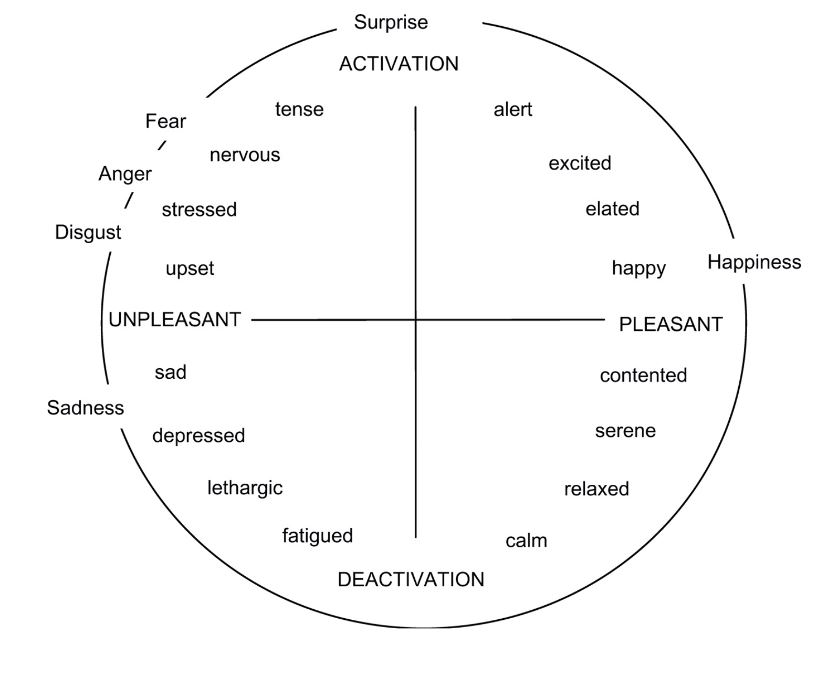
\includegraphics[width=0.6\textwidth]{imagens/russel.JPG}
\caption{\label{fig:russel}Modelo de Russel \cite{25}}
\end{figure}

\begin{figure}[!h]
\centering
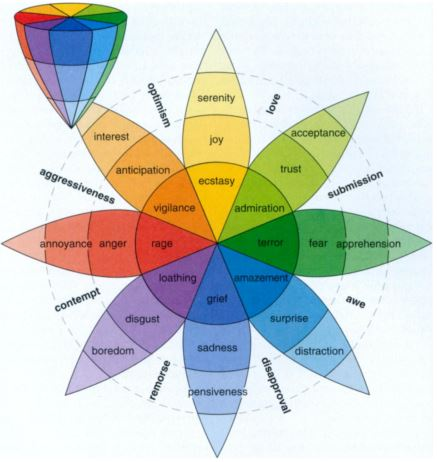
\includegraphics[width=0.7\textwidth]{imagens/plutchik.JPG}
\caption{\label{fig:plutchik}Modelo de Plutchik \cite{57}}
\end{figure}

% ==========================================================================================
\section{Aprendizado de Máquina}

O Aprendizado de Máquina (\textit{Machine Learning}, \textit{ML}) é uma subárea da Inteligência Artificial (\textit{Artificial Intelligence}, \textit{AI}). Inteligência Artificial foi o nome estabelecido \cite{12.23} para uma área denominada Inteligência Computacional, que consiste no estudo agentes inteligentes. Um agente é algo capaz de atuar num ambiente, enquanto um agente inteligente é um agente que atua no ambiente de forma inteligente, se apropriando de circunstâncias para alcançar um objetivo, possivelmente influenciando o ambiente, com capacidade para alterar esse objetivo, aprendendo com sua experiência e fazendo escolhas adequadas de acordo com suas limitações.

Tarefas de \textit{ML} costumam ser descritas em termos de como o sistema de aprendizado de máquina deve processar um exemplo \cite{53}. Um exemplo consiste numa coleção de recursos, de um objeto ou evento, que foram aferidos quantitativamente e que desejamos que seja processado por esse sistema. Costuma-se representar um exemplo como um vetor $x \in R^n$, onde cada coordenada $x_i$ do vetor $x$ é uma característica (\textit{feature}) desse vetor. Por exemplo, se $x$ representar uma imagem, cada $x_i$ pode ser o valor de um pixel dessa imagem.

Dentre as tarefas de \textit{ML}, duas tarefas comuns são a classificação e a regressão. A classificação busca descobrir a qual de $k$ classes possíveis um vetor $x$ pertence, produzindo uma função $f: R^n \rightarrow \{1, ..., k\}$, de modo que quando $y = f(x)$, o modelo atribui a uma entrada (\textit{input}) $x$ uma saída (\textit{output}) numérica de valor $y$ que representa uma categoria (classe). Na regressão, o pensamento é análogo, porém, ao final, o modelo não tenta encontrar a qual classe $x$ pertence, e sim predizer um valor (contínuo) para $f(x)$.

Diversos algoritmos de \textit{ML} foram investigados em trabalhos de SER \cite{20.7}, como Floresta Aleatória (\textit{Random Forest}, \textit{RF}) em \cite{20.10}, Árvore de Decisão \cite{20.11} (\textit{Decision Tree}), Máquinas de Vetor de Suporte \cite{20.13} (\textit{Support Vector Machines}, \textit{SVM}), K-vizinhos mais próximos \cite{20.15} (\textit{K-Nearest Neighbors}, \textit{KNN}) e Classificador de Aumento de Gradiente [20.16 (\textit{Gradient Boosting Classifier}, \textit{GBC}).

% ==========================================================================================
\section{Deep Learning e Redes Neurais}

Aprendizado Profundo (\textit{Deep learning}, \textit{DL}) é um tipo específico de ML \cite{53}. Algoritmos de ML citados no parágrafo anterior - conhecidos como algoritmos tradicionais - costumam funcionar bem em uma grande variedade de problemas importantes. Entretanto, não costumam ter desepenho tão bom em problemas que envolvem reconhecimento de fala ou de objetos. O desenvolvimento do \textit{DL} foi motivado, em parte, pela falha desses algoritmos tradicionais em generalizar bem para essas tarefas de IA.

Dada essa necessidade de explorar modelos mais robustos, alguns trabalhos estudaram o impacto de algoritmos de \textit{DL} no reconhecimento de emoção na voz \cite{12.12} \cite{12.16}.

\begin{figure}[!h]
\centering
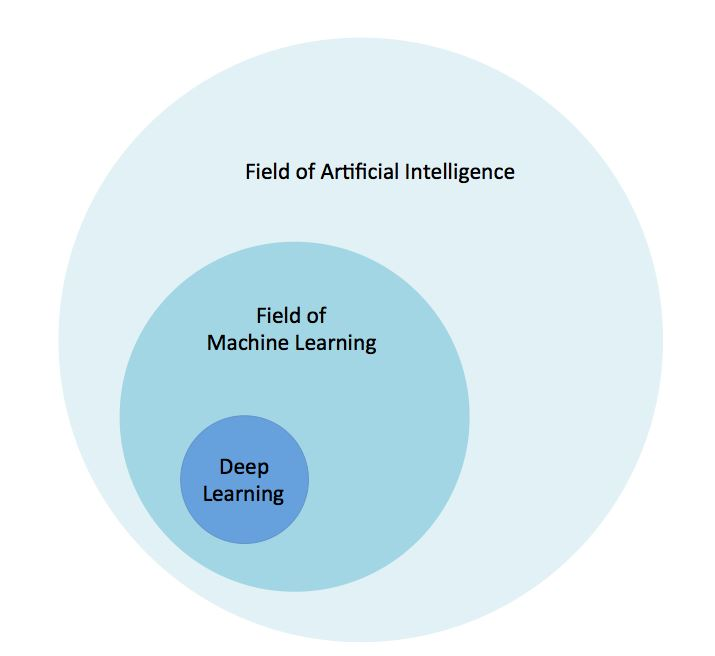
\includegraphics[width=0.5\textwidth]{imagens/ia-ml-dl.JPG}
\caption{\label{fig:ia-ml-dl}Relação entre \textit{IA}, \textit{ML} e \textit{DL}}

\author{Fonte: Retirada de \cite{58}}
\end{figure}

Redes Multicamadas de Perceptrons (\textit{Multilayer Perceptron}, \textit{MLP}) são a pedra fundamental na construção de modelos de \textit{DL}, conhecidos como Redes Neurais (\textit{Neural Networks}, \textit{NN}). O Perceptron é uma unidade (Figura \ref{fig:perceptron}) composta por valores (pesos) $wi$ e uma função de ativação $f$,  que recebe as \textit{fetures}, realiza uma operação matemática entre $wi,xi$, aplica a função de ativação $y = f(x,w)$ e emite esse resultado como \textit{output}.

Podemos realizar o mapeamento de vários Perceptrons, recebendo as \textit{features} e preoduzindo \textit{outputs}, ao longo de camadas, onde cada camada atua como \textit{input} para a próxima camada, e assim sucessivamente, até chegar a um \textit{output} final, assim, temos uma \textit{MLP} (Figura\footnote{Imagem adaptada, gerada em \url{http://alexlenail.me/NN-SVG/index.html}}\ref{fig:mlp}). A camada inicial é chamada de camada de entrada (\textit{input layer}), as camadas intermediárias são chamadas de camdas ocultas (\textit{hidden layers}) e à camada final chamamos camada de saída (\textit{output layer}). Compreendendo uma rede neural como um conjunto de nós e arestas, cada nó da rede será chamado de neurônio.

\begin{figure}[!ht]
\centering
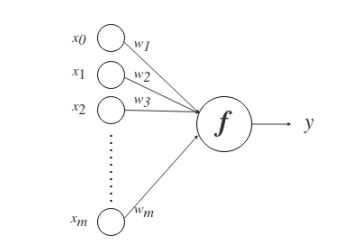
\includegraphics[width=0.6\textwidth]{imagens/perceptron.png}
\caption{\label{fig:perceptron}Exemplo de Perceptron}

\author{Fonte: Retirado de \cite{12}}
\end{figure}

\begin{figure}[!h]
\centering
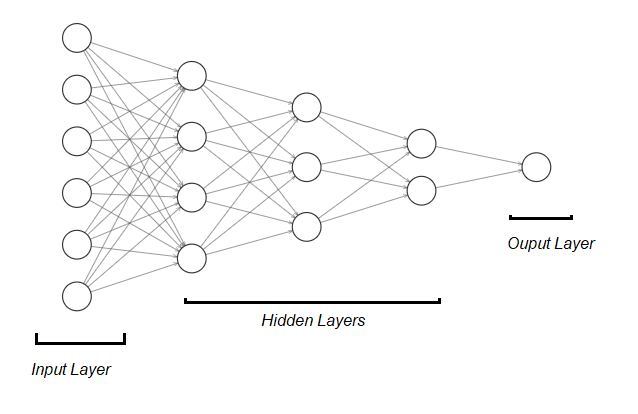
\includegraphics[width=0.75\textwidth]{imagens/mlp02.png}
\caption{\label{fig:mlp}Exemplo de arquitetura \textit{MLP}}

\end{figure}

% ------------------------------------------------------------------------------------------
\subsection{Redes Neurais Profundas}

Nosso cérebro tem uma grande capacidade de generaliação, o que nos ajuda a raciocinar de forma indutiva e é o primeiro passo do nosso aprendizado \cite{32}. Redes neurais são capazes de aprender relações não-lienares complexas e criar relações entre \textit{input} e \textit{output}, formando sistemas utilizados em várias áreas de \textit{ML}, e \textit{SER} não é uma exceção \cite{32.74}.

Com base no conceito e organização de uma rede neural, o conjunto formado pela disposição dos neurônios, pesos e funções de ativação pode ser organizado de forma a criar diferentes arquiteturas\footnote{Exemplos visuais de diversas arquiteturas de DL: \url{https://www.asimovinstitute.org/neural-network-zoo/}}, que ao longo do tempo se mostraram eficientes para generalizar bem em certas áreas de conhecimento. Diremos que uma rede neural se torna uma Rede Neural Profunda (\textit{Deep Neural Network}, \textit{DNN}) (Figura\footnote{Gerada em \url{http://alexlenail.me/NN-SVG/index.html}} \ref{fig:exarqdnn}) quando possue grande quantidade de neurônios e camadas ocultas em sua arquitetura, embora não haja um valor específico que a habilite a se tornar profunda ao superá-lo.

\begin{figure}[!h]
\centering
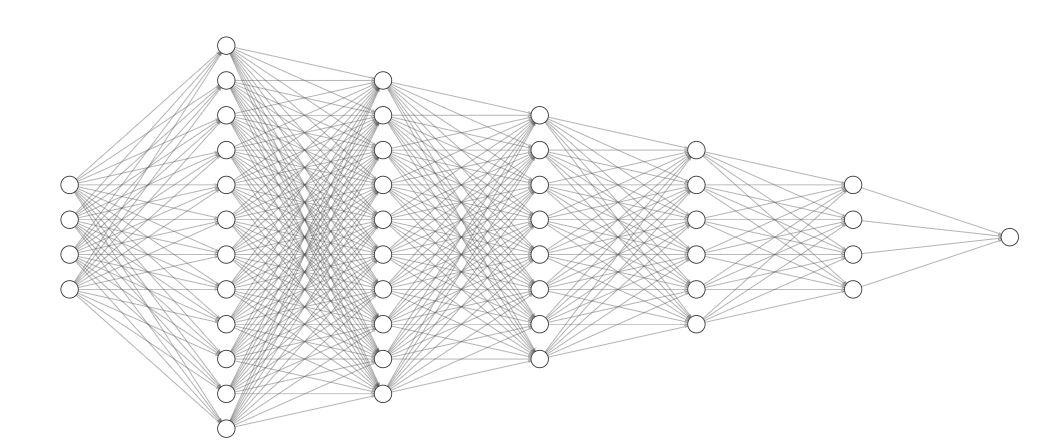
\includegraphics[width=1.0\textwidth]{imagens/ex-dnn.JPG}
\caption{\label{fig:exarqdnn}Exemplo de arquitetura \textit{DNN}}
\end{figure}

A seguir, abordaremos duas dessas arquiteturas que se mostram importantes para este trabalho: Redes Neurais Convolucionais e Autoencoder.

% ------------------------------------------------------------------------------------------
\subsection{Redes Neurais Convolucionais}

Redes Neurais Convolucionais\footnote{Introduzido em 1989 por Y. LeCun \textit{et al.}} (\textit{Convolutional Neural Networks}, \textit{CNN}), também conhecidas como Redes Convolucionais, são um tipo de rede neural especializada para processar dados que tenha uma topologia semelhante a um formato de grade. Dados como esses podem ser, por exemplo, imagens ou séries temporais. Poderíamos interpretar uma leitura numa série temporal num instante $t$ como uma coluna, e, assim, acumular horizontalmente essas leituras ao longo do tempo criando uma estrutura que atenda a esse padrão de gradem. Enquanto numa imagem, podemos interpretar os valores dos pixels como elementos que formam essa mesma estrutura. Um exemplo de uma arquitetura de \textit{CNN} pode ser observado na Figura\footnote{Gerada em \url{http://alexlenail.me/NN-SVG/LeNet.html}} \ref{fig:exarqcnn}.

O nome convolucional vem da operação de Convolução, uma operação linear entre duas funções $f$ e $g$ que produzem uma terceira função $f*g$ e que expressa como o formato de $f$ é influenciado por $g$. A operação de convolução é definida como:

\begin{equation}
(f*g)(t) \coloneqq \int^{-\infty}_{\infty}{f(a) * g(t - a) \partial{da}}
\end{equation}

Costumeiramente, nos referimos a convolução apenas através de $(f*g)(t)$, onde $f$ é nosso \textit{input}, $g$ será o nosso filtro (\textit{kernel}),  e o resultado (\textit{output}) da convolução costuma ser chamado de mapa de características (\textit{feature map}). Um exemplo de convolução pode ser observado na Figura \footnote{Imagem retirada de \url{https://courses.cs.washington.edu/courses/cse446/22wi/sections/08/convolutional_networks.html}} \ref{fig:2dconv}. Perceba que \textit{output} foi obtido movendo (deslizando) o \textit{kernel} ao longo das linhas e colunas do \textit{input}, realizando, a cada iteração, a soma do produto dos elementos sobrepostos entre o \textit{input} e o \textit{kernel}.

\begin{figure}[!h]
\centering
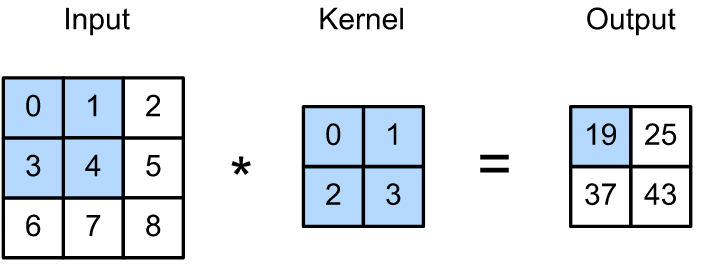
\includegraphics[width=0.7\textwidth]{imagens/2dconv.png}
\caption{\label{fig:2dconv}Exemplo de Convolução}
\end{figure}

\begin{figure}[!h]
\centering
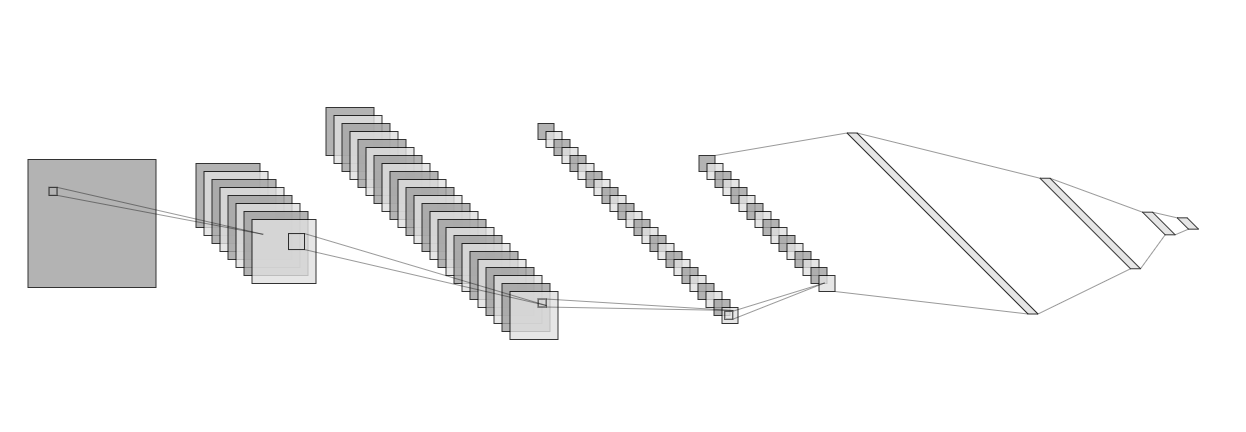
\includegraphics[width=1.0\textwidth]{imagens/ex-cnn.png} % https://towardsdatascience.com/applied-deep-learning-part-3-autoencoders-1c083af4d798
\caption{\label{fig:exarqcnn}Exemplo de arquitetura \textit{CNN}}
\end{figure}

Redes Neurais Convolucionais são populares em trabalhos envolvendo SER \cite{37.125} \cite{37.126} \cite{37.127} \cite{37.128}, e sua capacidade de generalização de características se mostra superior a abordagens puras de \textit{DNN} \cite{37.50}.

% ------------------------------------------------------------------------------------------
\subsection{Codificador Automático}

Um Codificador Automático (\textit{Autoencoder}, \textit{AE}) é uma rede neural criada para tentar reproduzir o seu \textit{input} no seu \textit{output}. Podemos descrever um \textit{AE} como um conjunto de funções $f, f'$ de modo que, dado um input $x$, queremos $f'(f(x)) = x' \approx x$, onde $f$ realiza a codificação (\textit{encoding}) de $x$ e $f'$ realiza a decodificação (\textit{decoding}) do resultado $f(x)$. Assim, um \textit{AE} é uma rede neural composta por um \textit{encoder} e um \textit{decoder} (Figura\footnote{Imagem adaptada, gerada em \url{http://alexlenail.me/NN-SVG/LeNet.html}} \ref{fig:exarqae}) que tenta reproduzir uma função de identidade.

O resultado da etapa de \textit{encoding} costuma ter uma dimensionalidade menor do que a do dado de entrada. O espaço composto por dados codificados (\textit{encoded}) é chamado de Espaço Latente (\textit{Latent Space}), um espaço composto por representações significativas dos dados, contendo informações sobre cada amostra que possivelmente não estariam visíveis nas representações de alta dimensionalidade \cite{60}.

Entretanto, \textit{Autoencoder}s não podem simplesmente aprender a generalizar $f'(f(x)) = x$ para todo tipo de dado, ao invés disso, são impostas restrições para que consigam esse tipo de generalização apenas para os dados relevantes a sua tarefa. Forçando o modelo a priorizar características que devem ser aprendidas, por vezes, ele aprende propriedades úteis sobre os dados.

Tradicionalmente, \textit{Autoencoder}s foram utilizados para reduzir a dimensionalidade de dados (\textit{dimensionality reduction}) ou para aprender características (\textit{feature learning}) sobre os dados. Atualmente, \textit{AE} são bastante utilizados como peça fundamental em Redes Generativas Adversariais \footnote{Introduzido em 2014 por Ian J. Goodfellow \textit{et al.}. Disponível em \url{https://arxiv.org/abs/1406.2661}} (\textit{Generative Adversarial Network}, \textit{GAN}) e \textit{Autoencoder}s Variacionais\footnote{Introduzido em 2013 por Diederik P Kingma e Max Welling. Disponível em \url{https://arxiv.org/abs/1312.6114}} (\textit{Variational Autoencoder}, \textit{VAE}).

\begin{figure}[!h]
\centering
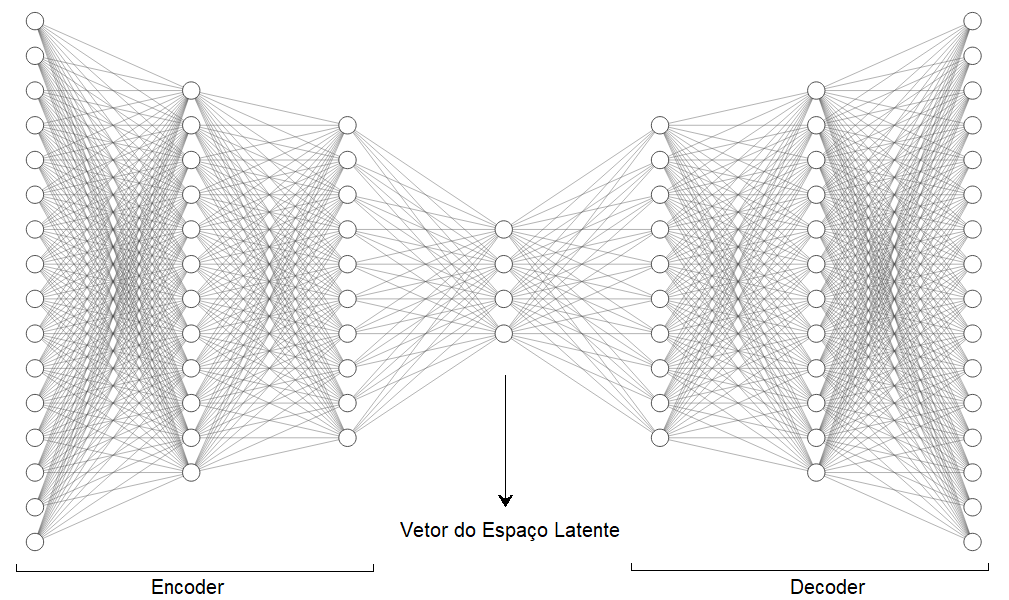
\includegraphics[width=1.0\textwidth]{imagens/ex-ae.PNG}
% \caption{\label{fig:exarqae}Exemplo de arquitetura \textit{AE}, com \textit{encoder}, \textit{decoder} e vetor do espaço latente}
\caption{\label{fig:exarqae}Exemplo de arquitetura \textit{AE}}
\end{figure}

% ==========================================================================================
\section{Abordagem: Supervisionada vs. Não Supervisionada}

No processo de criação de modelos de \textit{ML}, uma vez definida a arquitetura, a rede irá começar a aprender com os dados de forma iterativa. A etapa onde o modelo começa a ver os \textit{inputs} e tentar inferir a classe é chamada de treinamento (\textit{training}). Duas abordagens tradicionais para esse momento são a Aprendizagem Supervisionada (Supervised Learning) e a Aprendizagem Não Supervisionada (Unsupervised Learning).

% ------------------------------------------------------------------------------------------
\subsection{Abordagem Supervisionada}\label{supervisionada}

Para a primeira, é necessário que os dados já estejam rotulados com a classe (\textit{label}) a qual cada registro de pertence. Por exemplo, ao utilizar uma base de dados que envolve imagens, pode ser trivial etiquetar os dados com base no objeto que aparece naquela imagem (e.g.: ou gato ou cachorro). Para emoções essa atividade irá demandar pessoas especializadas e capacitadas. Uma pesquisa \cite{32} recente (2021) aponta essa dificuldade na área de \textit{SER}, pois mesmo quando há variedade de conjuntso de dados (\textit{datasets}) diferentes, estes podem apresentar poucas classes, poucos registros por classe ou ambos.

Sejam $X, Y$, conjuntos de \textit{inputs} e \textit{outputs}, respectivamente, $X=\{x_i, ..., x_n\}$ e $Y=\{y_i, ..., y_n\}$, onde o $y_i$ é a classe de $x_i$, podemos generalizar a etapa de treinamento como seguinte fluxo $\forall x_i \in X' \subset X$:

Seja $f: X \rightarrow Y,$ tal que $f(x) = y$, então,

\begin{enumerate}
    \item O modelo $f$ é apresentado a um dado $x_i$ e produz um resultado $f(x_i) = y_i'$;
    \item É calculado um erro $d_i = d(y_i, y_i')$ entre o resultado apresentado e o resultado esperado;
    \item $d_i$ É utilizado para atualizar os parâmetros de $f$;
    \item O processo é repetido para o próximo exemplo $x_{i+1}$.
\end{enumerate}

A etapa de treinamento costuma ser serguida pela etapa de testes (\textit{tests}), onde o modelo é exposto aos $x_j \in (X \setminus X')$ e, a partir daí, são calculadas métricas para aferir o desempenho de $f$.

Cabe observar que $f$ não precisa ser injetora, uma vez que mais de um $x_i$ pode pertencer a mesma classe $y_i$.

\subsection{Abordagem Não Supervisionada}

Para uma abordagem não supervisionada, os modelos são apresentados a um conjunto de dados sem rótulos e tentam aprender características importantes da sua estrutura. A distinção entre supervisionado e não supervisionado costuma se dar pela presença ou não da classe (\textit{target}) daqueles dados. Note que é possível aplicar uma abordagem não supervisionada a um \textit{dataset} mesmo quando a classe é conhecida, basta excluí-la do processo de treinamento do modelo.

Alguns casos de uso de \textit{Unsupervised Learning} incluem: (1) Formação de conjuntos (\textit{clustering}); (2) \textit{Feature Learning}; (3) Redução de dimensionalidade; (4) Automatizar a rotulação de amostras; (5) Aprender sobre o \textit{dataset} através de análise exploratória (\textit{Exploratory Data Analysis}, \textit{EDA}).

Trabalhos envolvendo aprendizado não supervisionado apontam as capacidades do \textit{AE} tanto para \textit{feature learning} \cite{35.16} \cite{35.17} quanto para redução de dimensionalidade \cite{35.18} \cite{35.19}.

% ==========================================================================================
\section{Base de Dados}\label{section:basesdedados}

Para modelar a intensidade da emoção, uma das dificuldades é a falta de dados rotulados \cite{18}. Tradicionalmente, em áreas como visão computadional ou reconhecimento de voz, os \textit{datasets} chegam a ter milhões de registros, como, por exemplo: ImageNet\footnote{Disponível em \url{https://www.image-net.org/about.php}} (imagem) com  mais de 14 milhões e Google AudioSet\footnote{Disponível em \url{http://research.google.com/audioset/}} (áudio) com mais de 2 milhões de amostras. Podemos ver um comparativo na Tabela \ref{table:comparativodbs} entre datasets populares \cite{32} em trabalhos de \textit{SER}: AudioSet, Berlin Database of Emotional Speech (EMO-DB) \cite{32.55}, Danish emotional speech database (DES) \cite{32.56}, The Ryerson Audio-Visual Database of Emotional Speech and Song (RAVDESS) \cite{32.57}, Toronto Emotional Speech Set (TESS) \cite{32.58} e Crowd-Sourced Emotional Multimodal Actors Dataset (CREMA-D) \cite{32.59}.

\begin{table}[!ht]\label{table:comparativodbs}
\centering
\caption{Comparativos entre \textit{datasets} populares para \textit{SER}}
    \begin{tabular}{|l|c|c|c|}
    \hline
        Nome & Quantidade de amostras & Duração Média (s) & Português?  \\ \hline
        EMO-DB  & 700 & 2,8 & Não  \\ \hline
        DES  & 210 & 2,7 & Não  \\ \hline
        RAVDESS  & 2496 & 3,7 & Não  \\ \hline
        TESS  & 2800 & 2,1 & Não  \\ \hline
        CREMA-D  & 7442 & 2,5 & Não  \\ \hline
    \end{tabular}
\end{table}

Não obstante nenhum destes ser em português, língua falada pela sexta\footnote{Disponível em \url{https://brasilescola.uol.com.br/geografia/populacao-mundial.htm}} maior população e nona\footnote{Disponível em \url{https://www.gov.br/funag/pt-br/ipri/publicacoes/estatisticas/as-15-maiores-economias-do-mundo}} maior economia do mundo, podemos observar com facilidade o quão distante estão do AudioSet, tanto em quantidade de amostras ($> 2.000.000$) quanto em duração média ($\approx 10s$).

Todos esses \textit{datasets} são simulados (\textit{simulated}), ou seja, os áudios são gravados a partir de pessoas treinadas lendo um texto e interpretando com emoções diferentes. Existem também datasets seminaturais (\textit{semi-natural}), composto tanto por atores como pessoas comuns lendo um roteiro; e os dito naturais (\textit{natural}), com áudios extraídos de programas de TV, centrais telefônicas, vídeos da internet e outros meios.

Também é comum que as amostras não apresentem ruídos ou alguma puluição sonora, o que as distancia de situações reais. Sistemais treinados neses datasets podem não ser bem sucedidos em situações reais \cite{32}. Há também \textit{datasets} gerados a partir da particiação de um usuário ou cliente de algum serviço, entretanto, este é informado da gravação, o que pode comprometer a qualidade do dado.

Outro problema é o efeito da cultura e da linguagem, onde ambos os fatores podem afetar a percepcão do sentimento na fala \cite{32}. A incerteza na anotação (categorização dos dados) representa mais um desafio para \textit{datasets} de \textit{SER}, uma vez que num discurso emocional, um participante pode rotular um enunciado com \textit{eufórico} e outro como \textit{raivoso}. Essa subjetividade torna a tarefa mais complexa e pode limitar a possibilidade de misturar os bancos de dados para criar superconjuntos de dados emocionais.

% ------------------------------------------------------------------------------------------
\subsection{Fusão de Domínios}

Dado esse cenário, podemos tentar utilizar uma ténica que permite fundir o conhecimento de vários conjuntos de dados organicamente para uma tarefa de aprendizado de máquina. Fusão de Domínios \cite{49}(\textit{Domain Fusion}) é uma técnica para aproveitar mais bases de dados e produzir informações mais robustas e úteis do que as fornecidas por uma única fonte de dados individualmente. Um exemplo de utilização de fusão de domínios pode ser observado em \cite{3} para tentar melhorar a generalização do seu modelo, e que percebeu uma melhora do desempenho em dados inéditos (distintos das amostras de treinamento e teste).

Uma vez que compreendemos, o processo de formação da fala, do seu emprego na tranmissão de emoções, formas de categorizá-las, como se dá um trabalho que envolve algoritmos de \textit{DL}, faz-se necessário conseguir uma massa de dados que possa ser utilizada para esta atividade. Neste trabalho, utilizaremos dois conjuntos de dados: VERBO e VIVAE.

% ------------------------------------------------------------------------------------------
\subsection{VERBO}

VERBO \cite{12.21} (\textit{Voice Emotion Recognition Database in Portuguese Language}),  é uma base de dados com 1176 arquivos em formato \textit{.wav}, publicada em 2018, criada no Instituto de Matemática e Ciências da Computação da Universidade de São Paulo, ICMC-USP, fomada por arquivos de áudio na língua portuguesa do Brasil, rotulados com emoções. É o primeiro \cite{21} dataset para \textit{SER} em português do Brasil.

Os áudios têm duração entre 2 e 5 segundos, gravados por doze atores brasileiros - seis homens e seis mulheres - de diferentes idades e regiões do país. Compreende quatorze enunciados (\textit{utterances}) validados por um profissional linguístico, acomodando todos os fonemas da língua portuguesa. Possui exemplos das 6 emoções básicas propostas pro Russel: (1) Alegria; (2) Nojo; (3) Medo; (4) Raiva; (5) Surpresa; (6) Tristeza. Por fim, foi adicionado um sétimo estado emocional, denomioado de (7) Neutro. A distribuição das classes pode ser observada na Tabela \ref{table:verbo}.

\begin{table}[!ht]\label{table:verbo}
\centering
\caption{Distribuição por classe das 1167 sentenças do \textit{dataset} VERBO}
    \begin{tabular}{|l|r|}
    \hline
        Classe & Total \\ \hline
        Raiva & 167  \\ \hline
        Nojo & 167  \\ \hline
        Medo & 166  \\ \hline
        Alegria & 166  \\ \hline
        Tristeza & 167  \\ \hline
        Surpresa & 167  \\ \hline
        Neutro & 167  \\ \hline
    \end{tabular}
\end{table}

% ------------------------------------------------------------------------------------------
\subsection{VIVAE}

VIVAE \cite{16} (\textit{Variably Intense Vocalizations of Affect and Emotion Corpus}) é uma base de dados com 1085 arquivos em formato \textit{.WAV}, publicada em 2020, criada por pesquisadores alemães e estadunidenses, formada por vocalizações não verbais.

Os áudios foram gravados por onze pessoas, compreendendo três sentimentos positivos e três negativos:

\begin{itemize}
    \item Positivos: Conquista (\textit{achievment/triumph}), prazer sexual (\textit{sexual pleasure}) e surpresa (\textit{positive surprise});
    \item Negativos: Raiva (\textit{anger}), medo (\textit{fear}) e dor física (\textit{physical pain}).
\end{itemize}

Todos foram gravados com a intensidade variando entre baixa, moderada, forte e pico de emoção. A distribuiçao das intensidades pode ser observada na Tabela \ref{table:vivaeintensidade} e a das classes na Tabela \ref{table:vivae}.

\begin{table}[!ht]\label{table:vivaeintensidade}
    \centering
    \caption{Distribuição por intensidade das 1085 sentenças do \textit{dataset} VIVAE}
    \begin{tabular}{|l|r|}
    \hline
        Intensidade & Total  \\ \hline
        Baixa & 262  \\ \hline
        Moderada & 269  \\ \hline
        Forte & 272  \\ \hline
        Pico & 282  \\ \hline
    \end{tabular}
\end{table}

\clearpage

\begin{table}[!ht]\label{table:vivae}
\centering
\caption{Distribuição por classe das 1085 sentenças do \textit{dataset} VIVAE}
\begin{tabular}{|
>{\columncolor[HTML]{FFFFFF}}l |
>{\columncolor[HTML]{FFFFFF}}l |
>{\columncolor[HTML]{FFFFFF}}c |
>{\columncolor[HTML]{FFFFFF}}c |}
\hline
\multicolumn{1}{|c|}{\cellcolor[HTML]{FFFFFF}Sentimento} & \multicolumn{1}{c|}{\cellcolor[HTML]{FFFFFF}Intensidade} & \multicolumn{1}{c|}{\cellcolor[HTML]{FFFFFF}Quantidade} & Total                                         \\ \hline
\cellcolor[HTML]{FFFFFF}                                 & Baixa                                                    & 43                                                      & \cellcolor[HTML]{FFFFFF}                      \\ \cline{2-3}
\cellcolor[HTML]{FFFFFF}                                 & Moderada                                                 & 40                                                      & \cellcolor[HTML]{FFFFFF}                      \\ \cline{2-3}
\cellcolor[HTML]{FFFFFF}                                 & Pico                                                     & 39                                                      & \cellcolor[HTML]{FFFFFF}                      \\ \cline{2-3}
\multirow{-4}{*}{\cellcolor[HTML]{FFFFFF}Conquista}      & Forte                                                    & 39                                                      & \multirow{-4}{*}{\cellcolor[HTML]{FFFFFF}161} \\ \hline
\cellcolor[HTML]{FFFFFF}                                 & Baixa                                                    & 42                                                      & \cellcolor[HTML]{FFFFFF}                      \\ \cline{2-3}
\cellcolor[HTML]{FFFFFF}                                 & Moderada                                                 & 44                                                      & \cellcolor[HTML]{FFFFFF}                      \\ \cline{2-3}
\cellcolor[HTML]{FFFFFF}                                 & Pico                                                     & 44                                                      & \cellcolor[HTML]{FFFFFF}                      \\ \cline{2-3}
\multirow{-4}{*}{\cellcolor[HTML]{FFFFFF}Raiva}          & Forte                                                    & 44                                                      & \multirow{-4}{*}{\cellcolor[HTML]{FFFFFF}174} \\ \hline
\cellcolor[HTML]{FFFFFF}                                 & Baixa                                                    & 42                                                      & \cellcolor[HTML]{FFFFFF}                      \\ \cline{2-3}
\cellcolor[HTML]{FFFFFF}                                 & Moderada                                                 & 43                                                      & \cellcolor[HTML]{FFFFFF}                      \\ \cline{2-3}
\cellcolor[HTML]{FFFFFF}                                 & Pico                                                     & 46                                                      & \cellcolor[HTML]{FFFFFF}                      \\ \cline{2-3}
\multirow{-4}{*}{\cellcolor[HTML]{FFFFFF}Medo}           & Forte                                                    & 45                                                      & \multirow{-4}{*}{\cellcolor[HTML]{FFFFFF}176} \\ \hline
\cellcolor[HTML]{FFFFFF}                                 & Baixa                                                    & 42                                                      & \cellcolor[HTML]{FFFFFF}                      \\ \cline{2-3}
\cellcolor[HTML]{FFFFFF}                                 & Moderada                                                 & 47                                                      & \cellcolor[HTML]{FFFFFF}                      \\ \cline{2-3}
\cellcolor[HTML]{FFFFFF}                                 & Pico                                                     & 45                                                      & \cellcolor[HTML]{FFFFFF}                      \\ \cline{2-3}
\multirow{-4}{*}{\cellcolor[HTML]{FFFFFF}Dor}            & Forte                                                    & 51                                                      & \multirow{-4}{*}{\cellcolor[HTML]{FFFFFF}185} \\ \hline
\cellcolor[HTML]{FFFFFF}                                 & Baixa                                                    & 42                                                      & \cellcolor[HTML]{FFFFFF}                      \\ \cline{2-3}
\cellcolor[HTML]{FFFFFF}                                 & Moderada                                                 & 54                                                      & \cellcolor[HTML]{FFFFFF}                      \\ \cline{2-3}
\cellcolor[HTML]{FFFFFF}                                 & Pico                                                     & 52                                                      & \cellcolor[HTML]{FFFFFF}                      \\ \cline{2-3}
\multirow{-4}{*}{\cellcolor[HTML]{FFFFFF}Prazer}         & Forte                                                    & 54                                                      & \multirow{-4}{*}{\cellcolor[HTML]{FFFFFF}202} \\ \hline
\cellcolor[HTML]{FFFFFF}                                 & Baixa                                                    & 51                                                      & \cellcolor[HTML]{FFFFFF}                      \\ \cline{2-3}
\cellcolor[HTML]{FFFFFF}                                 & Moderada                                                 & 41                                                      & \cellcolor[HTML]{FFFFFF}                      \\ \cline{2-3}
\cellcolor[HTML]{FFFFFF}                                 & Pico                                                     & 46                                                      & \cellcolor[HTML]{FFFFFF}                      \\ \cline{2-3}
\multirow{-4}{*}{\cellcolor[HTML]{FFFFFF}Surpresa}       & Forte                                                    & 49                                                      & \multirow{-4}{*}{\cellcolor[HTML]{FFFFFF}187} \\ \hline
\end{tabular}
\end{table}



% ==========================================================================================
\section{Comparativo}

Fazendo uma intersecção entre as classes dos \textit{datasets}, conforme Tabela \ref{table:verbovsvivae}, percebemos apenas quatro classes em comum: Alegria, medo, raiva e surpresa. Realziando uma contagem das classes em comum, em ambas bases de dados (Tabela \ref{table:totalporclasse}), teremos 1364 amostras, o que representa uma quantidade maior do que alguns dos \textit{datasets} em \ref{table:comparativodbs}.

\begin{table}[!ht]\label{table:verbovsvivae}
\centering
\caption{Comparativo das emoções presentes no \textit{VERBO} e no \textit{VIVAE}}
    \begin{tabular}{|l|c|c|c|}
    \hline
        Emoção (Português / Inglês) & VERBO & VIVAE & Comum  \\ \hline
        - / \textit{Pain} & Não & Sim &    \\ \hline
        - / \textit{Pleasure} & Não & Sim &    \\ \hline
        Alegria / \textit{Achievement} & Sim & Sim & \textbf{X}  \\ \hline
        Medo / \textit{Fear} & Sim & Sim & \textbf{X}  \\ \hline
        Neutro / - & Sim & Não &    \\ \hline
        Nojo / – & Sim & Não &    \\ \hline
        Raiva / \textit{Anger} & Sim & Sim & \textbf{X}  \\ \hline
        Surpresa / \textit{Surprise} & Sim & Sim & \textbf{X}  \\ \hline
        Tristeza / - & Sim & Não &    \\ \hline
    \end{tabular}
\end{table}

Das amostras compreendidas pela combinação das bases de dados, 698 delas pertencem ao \textit{VIVAE}, o que significa que aproximadamente 51\% do nosso \textit{dataset}, tem, além das classes para emoções, classes para a intensidade.

Uma das metodologias da Fusão de Domínios \cite{49} é a Fusão de Dados Baseada em Aprendizado de Transferência (\textit{Transfer Learning-Based Data Fusion}). Uma das possibilidades que essa metodologia aborda compreende a fusão de bases de dados de natureza semelhante (\textit{Transductive Learning}) quando a tarefa é a mesma mas o domínio (ponto de partida) e o contra domínio (ponto de chegada) são distintos. Como o nosso caso, onde vamos partir da voz para chegar na intensidade da emoção. Por mais que estejam relacionados, são distintos. Por exemplo, em uma tarefa de predição de tráfego urbano, pode-se utilizar os dados da cidade A para tentar uma previsão sobre o tráfego na cidade B, caso os dados sobre B sejam limitados. 

\begin{table}[]\label{table:totalporclasse}
\centering
\caption{Total de amostras por classe em comum utilizando \textit{VERBO} e \textit{VIVAE}}
\begin{tabular}{lccc}
\hline
\rowcolor[HTML]{FFFFFF} 
\multicolumn{1}{|c|}{\cellcolor[HTML]{FFFFFF}}                             & \multicolumn{2}{c|}{\cellcolor[HTML]{FFFFFF}Base   de dados}                                            & \multicolumn{1}{c|}{\cellcolor[HTML]{FFFFFF}}                        \\ \cline{2-3}
\rowcolor[HTML]{FFFFFF} 
\multicolumn{1}{|c|}{\multirow{-2}{*}{\cellcolor[HTML]{FFFFFF}Sentimento}} & \multicolumn{1}{c|}{\cellcolor[HTML]{FFFFFF}VERBO} & \multicolumn{1}{c|}{\cellcolor[HTML]{FFFFFF}VIVAE} & \multicolumn{1}{c|}{\multirow{-2}{*}{\cellcolor[HTML]{FFFFFF}Total}} \\ \hline
\rowcolor[HTML]{FFFFFF} 
\multicolumn{1}{|l|}{\cellcolor[HTML]{FFFFFF}Alegria   (Achievment)}       & \multicolumn{1}{c|}{\cellcolor[HTML]{FFFFFF}166}   & \multicolumn{1}{c|}{\cellcolor[HTML]{FFFFFF}161}   & \multicolumn{1}{l|}{\cellcolor[HTML]{FFFFFF}327}                     \\ \hline
\rowcolor[HTML]{FFFFFF} 
\multicolumn{1}{|l|}{\cellcolor[HTML]{FFFFFF}Medo (Fear)}                  & \multicolumn{1}{c|}{\cellcolor[HTML]{FFFFFF}166}   & \multicolumn{1}{c|}{\cellcolor[HTML]{FFFFFF}176}   & \multicolumn{1}{l|}{\cellcolor[HTML]{FFFFFF}342}                     \\ \hline
\rowcolor[HTML]{FFFFFF} 
\multicolumn{1}{|l|}{\cellcolor[HTML]{FFFFFF}Raiva (Anger)}                & \multicolumn{1}{c|}{\cellcolor[HTML]{FFFFFF}167}   & \multicolumn{1}{c|}{\cellcolor[HTML]{FFFFFF}174}   & \multicolumn{1}{l|}{\cellcolor[HTML]{FFFFFF}341}                     \\ \hline
\rowcolor[HTML]{FFFFFF} 
\multicolumn{1}{|l|}{\cellcolor[HTML]{FFFFFF}Surpresa   (Surprise)}        & \multicolumn{1}{c|}{\cellcolor[HTML]{FFFFFF}167}   & \multicolumn{1}{c|}{\cellcolor[HTML]{FFFFFF}187}   & \multicolumn{1}{l|}{\cellcolor[HTML]{FFFFFF}354}                     \\ \hline
\end{tabular}
\end{table}

% \clearpage

% ==========================================================================================
\section{Processamento de Dados}

Para realizar tarefas de \textit{ML} a partir de arquivos de áudio, faz-se necessário convertê-los para uma forma passível de ingestão pelo modelo. Os arquivos das bases de dados estão em formato \textit{.wav} (encurtamento de \textit{WAVEform}), que não realiza compressão do som digital, mantendo-o mais próximo da expressão do som natural. Precisamos de uma forma de transformar os dados em uma representação que preserve suas características.

Podemos compreender um sinal como a variação de uma quantidade ao longo do tempo. No caso da voz, a variação da pressão do ar. Amostras da pressão do ar são aferidas ao longo do tempo, com uma determinada frequência. Temos um sinal unidimensional, ou seja, com uma única variável, a amplitude do som, distribuida ao longo do tempo (Figura \ref{fig:exsinalsom}).

No ato da fala, nossas pregas vocais oscilam um número de ciclos de acordo com o  seu comprimento, tamanho da massa de vibração envolvida e tensão. Essa oscilação também pode ser aferida uma quantidade de vezes por segundo, portanto, temos sua frequência.

Para transportar um sinal do domínio do tempo para o domínio da frequência, utiliza-se a Transformada de Fourier (\textit{Fourier Transform}, \textit{FT}), que irá decompor o sinal em seus componentes de frequências (Figura\footnote{Disopnível em \url{https://medium.com/analytics-vidhya/understanding-the-mel-spectrogram-fca2afa2ce53}} \ref{fig:fouriertransform}), realizada computacionalmente através da Transformada Rápida de Fourier (\textit{Fast Fourier Transform}, \textit{FFT}). % \footnote{No ano 2000 a \textit{FFT} foi incluída pela IEEE numa lista dos dez algoritmos mais influentes para o desenvolvimento e prática da ciência no século 20. Fonte: \textit{Guest Editors Introduction to the top 10 algorithms}. Disponível em \url{https://ieeexplore.ieee.org/document/814652/}})

\clearpage

\begin{figure}[!h]
\centering
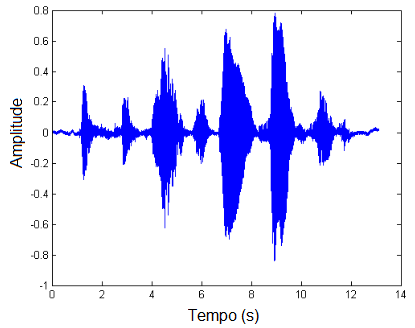
\includegraphics[width=0.75\textwidth]{imagens/exsinalsom.PNG}
\caption{\label{fig:exsinalsom}Exemplo de visualização de sinal sonoro, medindo a amplitude ao longo do tempo}

\author{Fonte: UNESP, Prinípios de Comunicações, 2013}
\end{figure}

\begin{figure}[!h]
\centering
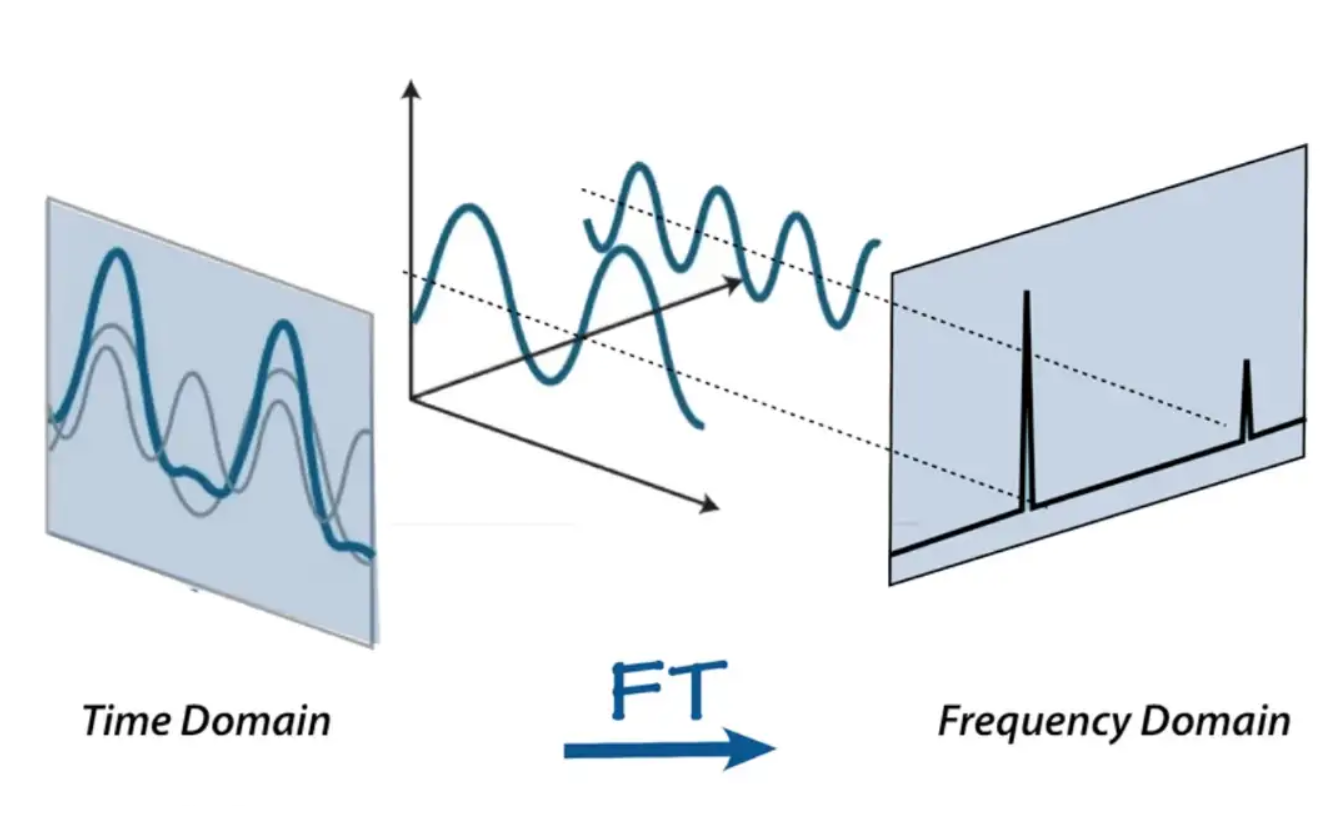
\includegraphics[width=0.6\textwidth]{imagens/ft.png}
\caption{\label{fig:fouriertransform}Ilustração da Transformada de Fourier}
\end{figure}

\clearpage

Com o resultado da \textit{FFT} de uma amostra, podemos calcular o seu espectrograma (\textit{spectrogram}): Uma representação da densidade das frequências ao longo do tempo. Entretanto, como humanos não compreendem todo o espectro sonoro \cite{62}, será aplicada uma normalização às frequências, e calcularemos o Espectrograma de Mel (\textit{Mel-Spectrogram}). Na Figura\footnote{Disponível em \url{https://medium.com/analytics-vidhya/understanding-the-mel-spectrogram-fca2afa2ce53}} \ref{fig:specvsmelespectrograma}, podemos observar a normalização das frequências (eixo vertical).

% https://towardsdatascience.com/learning-from-audio-the-mel-scale-mel-spectrograms-and-mel-frequency-cepstral-coefficients-f5752b6324a8
A normalização em questão, é a normalização pela escala de Mel (\textit{Mel Scale}). Uma escala construída para tornar tons equidistantes perceptivelmente equidistantes ao ouvido humano. A Escala de Mel é dada por:

\begin{equation}
    m(f) = 1127 * \log_e{(1 + \frac{f}{700})}
\end{equation}

\textit{Mel-Spectrogram} tem sido amplamente utilzada em problemas de \textit{SER}, como \cite{32.25} \cite{32.30}, e em \cite{32.31} e \cite{32.32}, que também utilizam \textit{CNN}s e ténicas de \textit{Autoencoder}.

Outro atributo observado na literatura são os Coeficientes Cepstrais de Frequência Mel (\textit{Mel Frequency Cepstral Coefficients}, \textit{MFCCs}). Um \textit{MFC} é uma representação de curto prazo do espectro de potência de um som, assim, \textit{MFC}s são os coeficientes que formam um \textit{MFCC} coletivamente. Calcular o \textit{MFCC} consiste em aplicar a Transformada Discreta do Cosseno (\textit{Discrete Cosine Transform}, \textit{DCT}) ao \textit{Mel-Spectrogram}. Podemos compreender o \textit{MFCC} como uma compressão \cite{64} do \textit{Mel Spectrogram}. Podemos observar um comparativo entre o resultado de um Mel-Spectrogram e um MFCC para uma mesma amostra na Figura \ref{fig:melspecvsmfcc}. Também encontramos trabalhos que utilizam \textit{MFCC}s em \cite{32.79} e \cite{32.89}, cujas arquiteturas contém uma CNN e uma GAN, respectivamente.

\clearpage

\begin{figure}[!h]
\centering
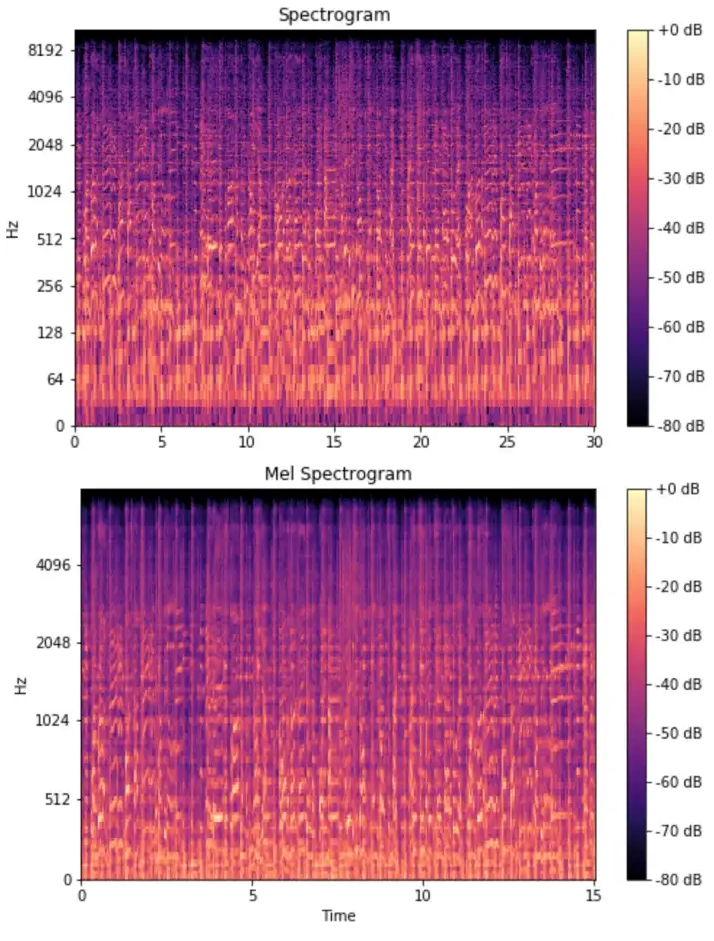
\includegraphics[width=0.55\textwidth]{imagens/espectrograma-vs-mel-espectrograma.png}
\caption{\label{fig:specvsmelespectrograma}Exemplos de Espectrograma e Espectrograma de Mel}
\end{figure}

\begin{figure}[!h]
\centering
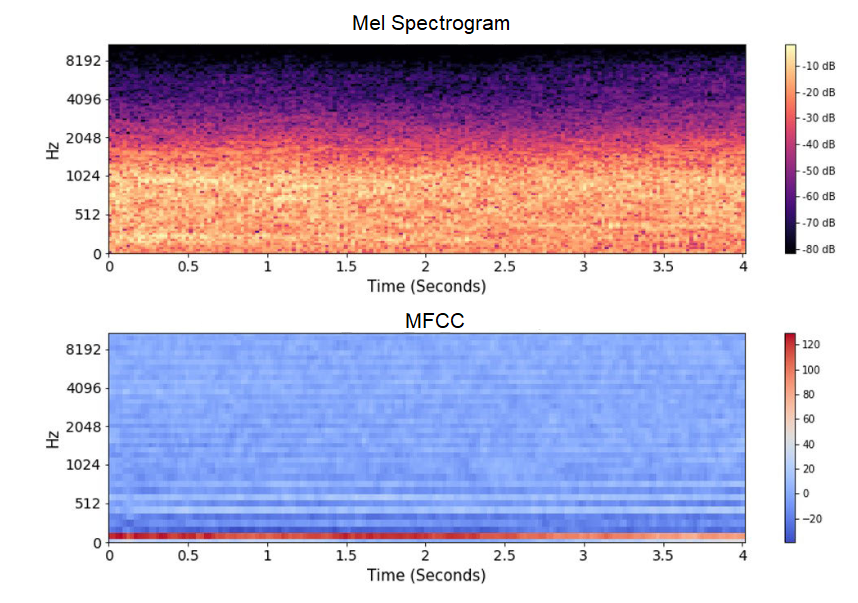
\includegraphics[width=0.7\textwidth]{imagens/melspec-vs-mfcc.PNG}
\caption{\label{fig:melspecvsmfcc}Espectrograma de Mel e MFCC de uma mesma amostra sonora}

\author{Fonte: Imagem adaptada de \cite{64}}
\end{figure}

% ==========================================================================================
\section{Métricas}\label{sec:metricas}

Na lista abaixo temos variáveis utilizadas para calcular as métricas de avaliação do desempenho de modelos de \textit{ML}:

\begin{itemize}
    \item Verdadeiros Positivos (VP) ou \textit{True Positive} (\textit{TP}): Classificação correta da classes positiva;
    \item Verdadeiros Negativos (VN) ou \textit{True Negative} (\textit{TN}): Classificação correta da classes negativa;
    \item Falsos Positivos (FP) ou \textit{False Positive} (\textit{FP}): Erro onde o modelo previu uma classe positiva, quando o valor real pertencia a classe negativa;
    \item Falsos Negativos (FN) ou \textit{False Negative} (\textit{FN}): Erro onde o modelo previu uma classe negativa, quando
o valor real pertencia a classe positiva.
\end{itemize}

Com essas variáveis, podemos calcular as seguintes métricas:

\begin{itemize}
    \item Acurácia (\textit{Accuracy}): Indica a performance geral do modelo.
        \begin{equation}
        \frac{VP + VN}{VP+FP+FN+FN}
        \end{equation}
    \item Precisão (\textit{Precision}): Dentre as classificações positivas que o modelo fez, quais foram corretas.
        \begin{equation}
        \frac{VP}{VP+FP}
        \end{equation}
    \item Sensibilidade (\textit{Recall}): Dentre todas as classificações positivas esperadas, quantas foram corretas.
        \begin{equation}
        \frac{VP}{VP+FN}
        \end{equation}
    \item \textit{F1-Score}: Média harmônica entre precisão e sensibilidade.
        \begin{equation}
        2 * \frac{precision  * recall}{precision + recall}
        \end{equation}
\end{itemize}

No âmbito de comparação de imagens, podemos citar o Índice de Similaridade Estrutural (\textit{Structural similarity}, \textit{SSIM}), que mede a similaridade entre duas imagens digitais. \textit{SSIM} é um modelo baseado na percepção, que considera a degradação da imagem como uma mudança percebida na sua informação estrutural, ao mesmo tempo em que incorpora fenômenos perceptivos de luminância e contraste, fornecendo um índice de qualidade para uma imagem (local). Tendo em vista o bom desempenho do sistema visual humano \cite{61} em perceber a estrutura visuais, o \textit{SSIM} se torna próximo da qualidade subjetiva que atribuimos a imagens.

O \textit{SSIM} é calculado em porções (janelas) da imagem, de modo que o índice entre duas janelas $x$ e $y$ de tamanho comum $NxN$ é dado por:

\begin{equation}
    % https://www.mathworks.com/help/images/ref/ssim.html
    SSIM(x,y) = [l(x,y)]^\alpha * [c(x,y)]^\beta * [s(x,y)]^\gamma
\end{equation}

Onde,

\begin{equation}
    l(x,y) = \frac{(2 * \mu_x * \mu_y) + C_1}{\mu_x^2 + \mu_y^2 + C_1}
\end{equation}

\begin{equation}
    c(x,y) = \frac{(2 * \sigma_x * \sigma_y) + C_2}{\sigma_x^2 + \sigma_y^2 + C_2}
\end{equation}

\begin{equation}
    s(x,y) = \frac{\sigma_{xy} + C_3}{(\sigma_x * \sigma_y) + C_3}
\end{equation}

E seus parâmetros, $\mu_x, \mu_y, \sigma_x, \sigma_y, \sigma_{xy}$, são as médias locais, desvios padrão e covariância cruzada para imagens $x, y$.

Quando $\alpha = \beta = \gamma = 1$ e $C3 = \frac{C2}{2}$, a equação fica simplificada da seguinte forma:

\begin{equation}
    SSIM(x,y) = \frac{(2 * \mu_x * \mu_y + C_1) * (2 * \sigma_{xy} + C_2)}{(\mu_x^2 + \mu_y^2 + C_1) * (\sigma_x^2 + \sigma_y^2 + C_2)}
\end{equation}

